% =====================================================================
% DECK SUPERADO. No usar para ensayar ni para sustentar.
% El deck vigente es beamer_defensa_v3.tex (41 paginas, LuaLaTeX).
% Este archivo se conserva solo como registro historico: NO lleva las
% correcciones posteriores (analisis por escenario con 3 semillas,
% etiquetado de la plausibilidad de GNNShap, tamanos de efecto).
% =====================================================================
% =====================================================================
% Presentacion de defensa (Beamer): REDISENO v2, estilo academico.
% Autores: Alejandro Gomez Huertas & Juan Diego Garzon Ovalle. UTP MISC 2026.
% Numeros = version corregida (post fix R1).
% Compilar:  pdflatex beamer_defensa_v2.tex  (dos veces, por el indice/TOC)
% =====================================================================
\documentclass[aspectratio=169,11pt]{beamer}
\usepackage[utf8]{inputenc}
\usepackage[T1]{fontenc}
\usepackage{lmodern}
\usepackage[spanish]{babel}
\usepackage{graphicx}
\usepackage{booktabs}
\usepackage{array}
\usepackage{tikz}
\usetikzlibrary{arrows.meta}
\graphicspath{{../tesis_latex/}}

% ------------------------------------------------ paleta institucional
\definecolor{navy}{HTML}{15263D}
\definecolor{navylt}{HTML}{223A5E}
\definecolor{teal}{HTML}{1C7293}
\definecolor{amber}{HTML}{E9A23B}
\definecolor{seafoam}{HTML}{2A9D8F}
\definecolor{coral}{HTML}{D9534F}
\definecolor{ink}{HTML}{1B2733}
\definecolor{muted}{HTML}{63748A}
\definecolor{panel}{HTML}{EEF3F8}

% ------------------------------------------------ tema
\usetheme{default}
\usefonttheme{professionalfonts}
\setbeamertemplate{navigation symbols}{}
\setbeamersize{text margin left=0.9cm,text margin right=0.9cm}

\setbeamercolor{normal text}{fg=ink}
\setbeamercolor{structure}{fg=teal}
\setbeamercolor{title}{fg=navy}
\setbeamercolor{frametitle}{fg=navy}
\setbeamercolor{itemize item}{fg=amber}
\setbeamercolor{itemize subitem}{fg=teal}
\setbeamercolor{enumerate item}{fg=teal}
\setbeamercolor{block title}{fg=white,bg=teal}
\setbeamercolor{block body}{fg=ink,bg=panel}
\setbeamercolor{block title alerted}{fg=white,bg=coral}
\setbeamercolor{block body alerted}{fg=ink,bg=panel}
\setbeamercolor{section in toc}{fg=navy}

\setbeamerfont{frametitle}{series=\bfseries,size=\large}
\setbeamerfont{title}{series=\bfseries}
\setbeamerfont{block title}{series=\bfseries,size=\small}
\setbeamertemplate{itemize item}{\small\raise0.5pt\hbox{\textbullet}}
\setbeamertemplate{itemize subitem}{\footnotesize\raise0.5pt\hbox{--}}
\setbeamertemplate{blocks}[rounded][shadow=false]

% ---- titulo de frame con regla teal (aire estructurado) ----
\setbeamertemplate{frametitle}{%
  \vspace{7pt}%
  {\usebeamerfont{frametitle}\usebeamercolor[fg]{frametitle}\insertframetitle}%
  \par\vspace{3pt}%
  {\color{teal}\rule{\textwidth}{1.1pt}}%
  \par\vspace{-5pt}%
}

% ---- footline institucional en tres segmentos ----
\setbeamercolor{fL}{fg=white,bg=navy}
\setbeamercolor{fC}{fg=white,bg=navylt}
\setbeamercolor{fR}{fg=white,bg=navy}
\setbeamertemplate{footline}{%
  \leavevmode%
  \hbox{%
    \begin{beamercolorbox}[wd=.30\paperwidth,ht=2.6ex,dp=1.15ex,leftskip=.5cm]{fL}%
      \tiny Gómez Huertas \textperiodcentered\ Garzón Ovalle%
    \end{beamercolorbox}%
    \begin{beamercolorbox}[wd=.46\paperwidth,ht=2.6ex,dp=1.15ex,center]{fC}%
      \tiny Estabilidad de XAI en GNNs para AML \textperiodcentered\ UTP 2026%
    \end{beamercolorbox}%
    \begin{beamercolorbox}[wd=.24\paperwidth,ht=2.6ex,dp=1.15ex,rightskip=.5cm]{fR}%
      \hfill\tiny\insertframenumber\,/\,\inserttotalframenumber%
    \end{beamercolorbox}%
  }\vspace{0pt}%
}

% ---- diapositiva divisoria de seccion, con indice resaltado ----
\setbeamertemplate{section in toc shaded}[default][30]
\AtBeginSection[]{%
  {\setbeamercolor{background canvas}{bg=navy}%
  \begin{frame}[plain,noframenumbering]%
    \vfill
    \hspace*{1.1cm}\begin{minipage}{0.86\textwidth}
      {\color{amber}\rule{1cm}{2.5pt}}\par\vspace{9pt}
      {\color{white!65}\normalsize Parte \insertsectionnumber}\par\vspace{3pt}
      {\color{white}\LARGE\bfseries \insertsectionhead}\par\vspace{16pt}
      {\setbeamercolor{section in toc}{fg=white}%
       \setbeamerfont{section in toc}{size=\small}%
       \tableofcontents[currentsection,hideallsubsections]}
    \end{minipage}
    \vfill
  \end{frame}}%
}

\title[Estabilidad XAI en GNNs]{Estabilidad de Métodos de Explicabilidad (XAI) en Graph Neural Networks para la Detección de Lavado de Dinero bajo Desbalance Extremo}
\author[Gómez \& Garzón]{Alejandro Gómez Huertas \and Juan Diego Garzón Ovalle}
\institute[UTP]{Director: Ph.D. Cristian Rosero Arias}
\date{Universidad Tecnológica de Pereira \textperiodcentered\ MISC \textperiodcentered\ 2026}

\begin{document}

% ===================================================================== PORTADA
{\setbeamercolor{background canvas}{bg=navy}
\begin{frame}[plain,noframenumbering]
\vspace{0.5cm}
{\color{amber}\footnotesize\bfseries UNIVERSIDAD TECNOLÓGICA DE PEREIRA \textperiodcentered\ MAESTRÍA EN INGENIERÍA EN SISTEMAS Y COMPUTACIÓN}\\[14pt]
{\color{white}\Large\bfseries Estabilidad de Métodos de Explicabilidad (XAI)\\[2pt] en Graph Neural Networks para la Detección\\[2pt] de Lavado de Dinero bajo Desbalance Extremo}\\[12pt]
{\color{amber}\rule{1.4cm}{2.5pt}}\\[12pt]
{\color{white}\normalsize\bfseries Alejandro Gómez Huertas \quad\textperiodcentered\quad Juan Diego Garzón Ovalle}\\[5pt]
{\color{white!80}\small Director: Ph.D. Cristian Rosero Arias}\\[2pt]
{\color{white!80}\small Facultad de Ingenierías \textperiodcentered\ Pereira, Colombia \textperiodcentered\ 2026}
\vfill
\end{frame}}

% ===================================================================== AGENDA
\begin{frame}{Contenido de la sustentación}
\vspace{2pt}
\begin{columns}[T]
\begin{column}{0.62\textwidth}
\begin{enumerate}
  \item[\textcolor{teal}{\textbf{1}}] \textbf{Problema y motivación}\\ {\small\color{muted}detección de lavado y la opacidad de las GNN}
  \item[\textcolor{teal}{\textbf{2}}] \textbf{Marco conceptual}\\ {\small\color{muted}arquitecturas, explicadores y las tres propiedades}
  \item[\textcolor{teal}{\textbf{3}}] \textbf{Metodología: dos ejes}\\ {\small\color{muted}Elliptic real + grafo sintético con \textit{ground-truth}}
  \item[\textcolor{teal}{\textbf{4}}] \textbf{Resultados}\\ {\small\color{muted}estabilidad, plausibilidad, fidelidad y sus relaciones}
  \item[\textcolor{teal}{\textbf{5}}] \textbf{Conclusiones}\\ {\small\color{muted}aportes, límites y trabajo futuro}
\end{enumerate}
\end{column}
\begin{column}{0.38\textwidth}
\setbeamercolor{block body}{bg=panel}
\begin{block}{Presentación a dos voces}
\footnotesize
\textbf{Alejandro}: contexto y metodología.\\[3pt]
\textbf{Juan Diego}: resultados y cierre.\\[6pt]
Duración objetivo: 33--36 min.
\end{block}
\end{column}
\end{columns}
\end{frame}

% ##################################################################### 1
\section{Problema y motivación}

\begin{frame}{El problema: detectar lavado sin caja negra}
\begin{columns}[T]
\begin{column}{0.56\textwidth}
\begin{itemize}
  \item El lavado mueve el \textbf{2--5\% del PIB mundial}; los sistemas por reglas generan \textbf{95--98\% de falsos positivos}.
  \item Las \textbf{GNN} modelan las transacciones como grafo y superan a lo tabular.
  \item \textbf{Pero son cajas negras}: en un entorno regulado, cada alerta debe ser justificable y reproducible.
\end{itemize}
\end{column}
\begin{column}{0.44\textwidth}
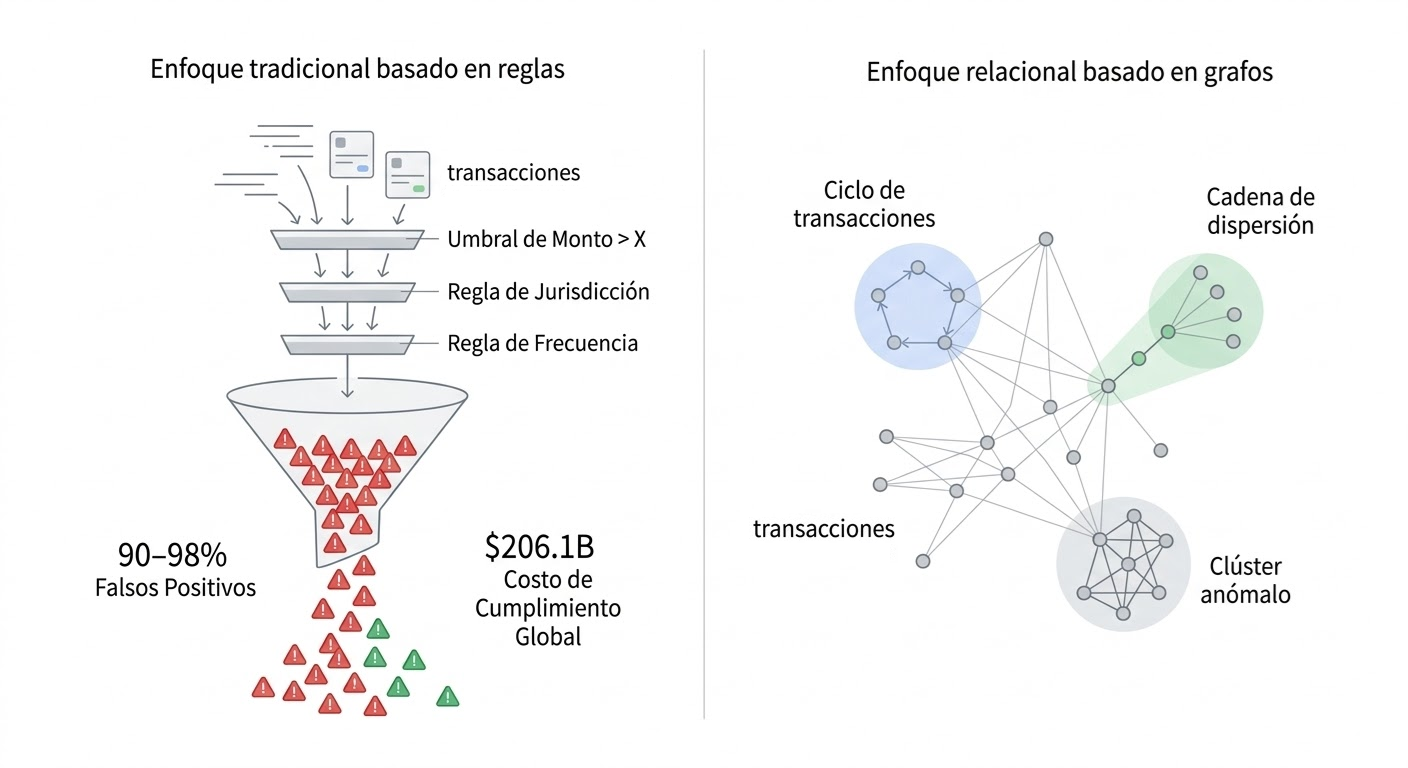
\includegraphics[width=\linewidth]{chapter_2/images_ch2/enfoques_moeny_laundering.png}
\end{column}
\end{columns}
\end{frame}

\begin{frame}{Pregunta de investigación y objetivos}
\begin{block}{Pregunta}
¿Cómo se comporta la \textbf{estabilidad} de los métodos XAI sobre GNNs para AML bajo desbalance, y qué combinación de arquitectura, explicador y balanceo optimiza la interpretación robusta y auditable?
\end{block}
\vspace{3pt}
\begin{columns}[T]
\begin{column}{0.5\textwidth}
\begin{itemize}
  \item[\textcolor{amber}{\textbf{O1}}] Degradación de la estabilidad con el desbalance.
  \item[\textcolor{amber}{\textbf{O2}}] Resiliencia de GCN, GraphSAGE, GAT, TAGCN.
\end{itemize}
\end{column}
\begin{column}{0.5\textwidth}
\begin{itemize}
  \item[\textcolor{amber}{\textbf{O3}}] Impacto de las estrategias de balanceo.
  \item[\textcolor{amber}{\textbf{O4}}] Matriz de recomendación técnica.
\end{itemize}
\end{column}
\end{columns}
\end{frame}

\begin{frame}{La brecha en el estado del arte}
\begin{columns}[T]
\begin{column}{0.5\textwidth}
\begin{block}{Lo que ya se sabía}
\begin{itemize}\small
  \item Las GNN superan a lo tabular (Weber 2019).
  \item TAGCN + SHAP con alto rendimiento (He 2026).
  \item Predicción y explicabilidad, por separado.
\end{itemize}
\end{block}
\end{column}
\begin{column}{0.5\textwidth}
\begin{alertblock}{Lo que faltaba}
\begin{itemize}\small
  \item La \textbf{estabilidad} de las explicaciones sobre grafos AML no se había evaluado sistemáticamente.
  \item Elliptic no tiene \textit{ground-truth} de tipología $\Rightarrow$ la plausibilidad no era medible.
\end{itemize}
\end{alertblock}
\end{column}
\end{columns}
\end{frame}

% ##################################################################### 2
\section{Marco conceptual}

\begin{frame}{Marco: redes de grafos y explicabilidad}
\begin{columns}[T]
\begin{column}{0.5\textwidth}
\textbf{\color{navy}4 arquitecturas GNN}
\begin{itemize}\small
  \item \textbf{GCN}: convolución espectral (1 salto)
  \item \textbf{GraphSAGE}: muestreo + agregación inductiva
  \item \textbf{GAT}: atención multi-cabeza
  \item \textbf{TAGCN}: filtros polinómicos de orden $K$
\end{itemize}
\end{column}
\begin{column}{0.5\textwidth}
\textbf{\color{navy}3 explicadores XAI (post-hoc)}
\begin{itemize}\small
  \item \textbf{GNNExplainer}: máscara por instancia
  \item \textbf{PGExplainer}: red generativa entrenada
  \item \textbf{GNNShap}: valores de Shapley por muestreo
\end{itemize}
\end{column}
\end{columns}
\end{frame}

\begin{frame}{Tres propiedades que no son lo mismo}
\begin{columns}[T]
\begin{column}{0.33\textwidth}
\begin{block}{Estabilidad}\small ¿La explicación se reproduce entre semillas y perturbaciones?\end{block}
\end{column}
\begin{column}{0.33\textwidth}
\begin{block}{Plausibilidad}\small ¿Señala el patrón real de lavado (\textit{ground-truth})?\end{block}
\end{column}
\begin{column}{0.33\textwidth}
\begin{block}{Fidelidad}\small ¿Refleja de verdad la decisión interna del modelo?\end{block}
\end{column}
\end{columns}
\vspace{10pt}
\begin{center}
\textcolor{amber}{\textbf{Tesis central:}} \textit{las tres son empíricamente independientes.}
\end{center}
\end{frame}

% ##################################################################### 3
\section{Metodología}

\begin{frame}{Qué produce, en concreto, un explicador}
\begin{columns}[T]
\begin{column}{0.46\textwidth}
\centering
\begin{tikzpicture}[scale=0.83, every node/.style={transform shape}]
  \tikzset{
    nodo/.style={circle,draw=muted,fill=white,minimum size=13pt,inner sep=0pt,line width=0.6pt},
    foco/.style={circle,draw=coral,fill=coral!22,minimum size=16pt,inner sep=0pt,line width=1.1pt},
    rel/.style={draw=amber,line width=2.1pt},
    irr/.style={draw=muted!45,line width=0.7pt}
  }
  \node[foco] (c) at (0,0) {};
  \node[nodo] (a) at (-1.55,0.95) {};
  \node[nodo] (b) at (-1.75,-0.55) {};
  \node[nodo] (d) at (1.55,0.9) {};
  \node[nodo] (e) at (1.7,-0.65) {};
  \node[nodo] (f) at (0.15,-1.6) {};
  \node[nodo] (g) at (-2.9,0.35) {};
  \node[nodo] (h) at (2.85,0.1) {};
  \draw[rel] (c) -- (a);
  \draw[rel] (c) -- (d);
  \draw[rel] (a) -- (g);
  \draw[irr] (c) -- (b);
  \draw[irr] (c) -- (e);
  \draw[irr] (c) -- (f);
  \draw[irr] (d) -- (h);
  \draw[irr] (b) -- (f);
\end{tikzpicture}
\\[3pt]
{\footnotesize \textcolor{coral}{$\bullet$} nodo a explicar \quad \textcolor{amber}{\rule[2pt]{9pt}{2pt}} aristas relevantes}
\end{column}
\begin{column}{0.52\textwidth}
\footnotesize
Ante una transacción marcada como ilícita, el explicador devuelve dos cosas:
\vspace{4pt}
\begin{enumerate}
  \item Una \textbf{máscara de aristas}: qué conexiones del vecindario sostienen la predicción.
  \item Un \textbf{ranking de \textit{features}}: qué atributos del nodo pesaron más, de los 166 disponibles.
\end{enumerate}
\vspace{6pt}
\begin{block}{}
Sobre eso se definen las tres preguntas:\\[3pt]
\textbf{Estabilidad}: ¿sale lo mismo al repetir?\\
\textbf{Plausibilidad}: ¿coincide con el patrón real?\\
\textbf{Fidelidad}: ¿es lo que el modelo usó?
\end{block}
\vspace{3pt}
{\color{muted}En Elliptic el vecindario tiene una mediana de $\sim$2 nodos, así que ahí solo el ranking de \textit{features} discrimina.}
\end{column}
\end{columns}
\end{frame}

\begin{frame}{Metodología: un diseño de dos ejes}
\begin{columns}[T]
\begin{column}{0.5\textwidth}
\begin{block}{Eje 1 \textperiodcentered\ Elliptic (real)}
\begin{itemize}\small
  \item Validez \textbf{externa}: transacciones reales.
  \item Sin \textit{ground-truth} $\Rightarrow$ solo estabilidad.
  \item Campo receptivo minúsculo ($\sim$2 nodos).
\end{itemize}
\end{block}
\end{column}
\begin{column}{0.5\textwidth}
\begin{block}{Eje 2 \textperiodcentered\ Sintético (propio)}
\begin{itemize}\small
  \item Validez \textbf{interna}: \textit{ground-truth} por nodo y arista.
  \item Permite medir plausibilidad y fidelidad.
  \item 4 tipologías estándar; 3 realizaciones.
\end{itemize}
\end{block}
\end{column}
\end{columns}
\end{frame}

\begin{frame}{Diseño factorial}
\begin{center}
{\color{teal}\Large\textbf{4}} arquitecturas \; $\times$ \; {\color{amber}\Large\textbf{3}} explicadores \; $\times$ \; {\color{seafoam}\Large\textbf{3}} balanceos \; $\times$ \; {\color{coral}\Large\textbf{5}} escenarios
\end{center}
\vspace{2pt}
\begin{center}\small = 60 configuraciones por eje \, $\times$ 3 explicadores para el estudio de estabilidad\end{center}
\vspace{6pt}
\begin{block}{Protocolo de robustez}
\small Estabilidad: 5 réplicas estocásticas por explicación. Inferencia (eje sintético): 3 semillas de modelo $\times$ 3 grafos, con Kruskal-Wallis, Wilcoxon e IC bootstrap.
\end{block}
\end{frame}

\begin{frame}{Eje 1: Elliptic Bitcoin Dataset}
\begin{columns}[T]
\begin{column}{0.54\textwidth}
\begin{itemize}\small
  \item 203.769 nodos \textperiodcentered\ 234.355 aristas \textperiodcentered\ 166 features \textperiodcentered\ 49 pasos.
  \item Ilícitas $\sim$2,2\% (razón $\sim$1:9 en el subconjunto etiquetado).
  \item Split temporal causal (train 1--34 / val 35--42 / test 43--49).
  \item Campo receptivo mediana $\sim$2 nodos $\Rightarrow$ solo el Spearman discrimina.
\end{itemize}
\end{column}
\begin{column}{0.46\textwidth}
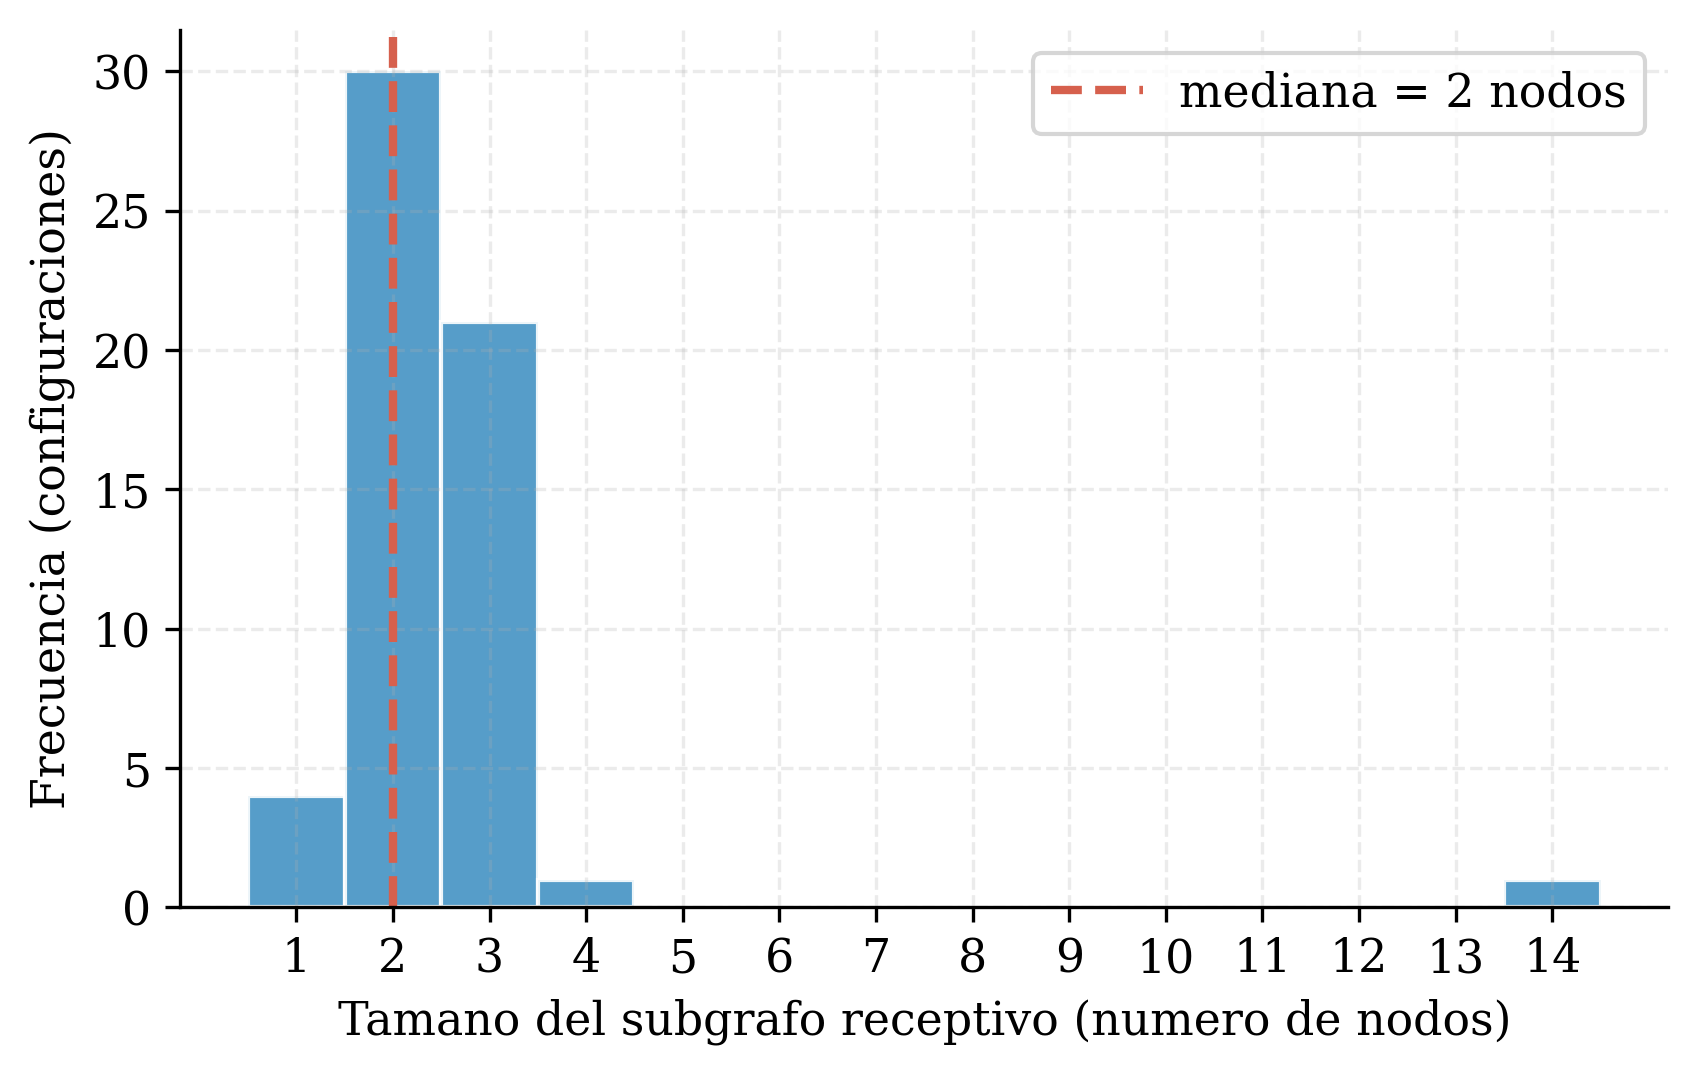
\includegraphics[width=\linewidth]{chapter_4/images_ch4/dispersion_elliptic.png}
\end{column}
\end{columns}
\end{frame}

\begin{frame}{Eje 2: grafo sintético con ground-truth}
\begin{columns}[T]
\begin{column}{0.54\textwidth}
\begin{itemize}\small
  \item \textbf{¿Por qué?} medir plausibilidad exige saber cuál subgrafo es el patrón: Elliptic no lo da.
  \item 4 tipologías: \textit{structuring}, \textit{layering}, \textit{fan-in}, \textit{fan-out}.
  \item Aristas distractoras + firma atenuada $\Rightarrow$ la métrica discrimina.
  \item \textit{Ground-truth} ciego al explicador; 3 realizaciones.
\end{itemize}
\end{column}
\begin{column}{0.46\textwidth}
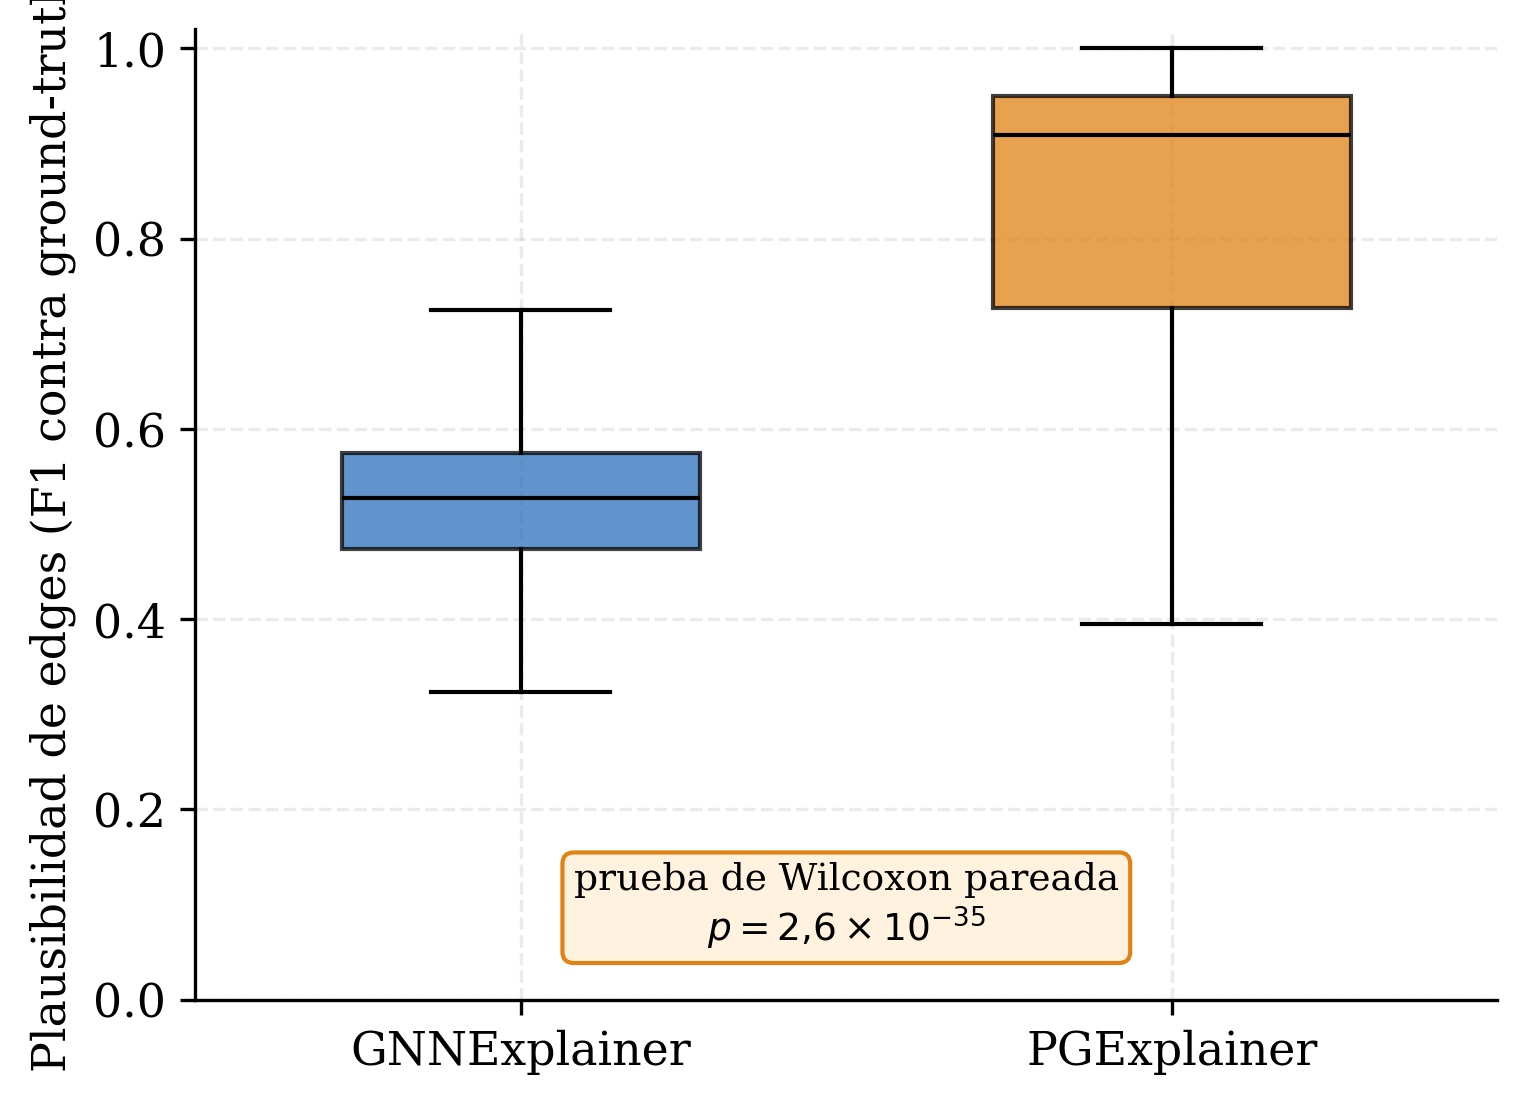
\includegraphics[width=\linewidth]{chapter_5/images_ch5/hallazgo_estrella.png}
\end{column}
\end{columns}
\end{frame}

\begin{frame}{Cómo se construyó el grafo sintético}
\begin{columns}[T]
\begin{column}{0.5\textwidth}
\footnotesize
\textbf{Decisiones que endurecen la prueba}
\begin{itemize}
  \item \textbf{Simetrización} de aristas: sin ella el campo receptivo cae a $\sim$2 nodos y la plausibilidad de subgrafo no es medible.
  \item \textbf{Aristas distractoras} ($n=3$ por nodo de patrón): sin ellas cualquier selección \textit{top-k} acertaría.
  \item \textbf{Firma de \textit{features} atenuada} de $+4$ a $+1{,}5$: evita que la tarea se resuelva sola.
\end{itemize}
\vspace{3pt}
{\color{muted}El \textit{ground-truth} se fija en la construcción, \textbf{antes} de correr ningún explicador.}
\end{column}
\begin{column}{0.5\textwidth}
\footnotesize
\textbf{Escala y replicación}
\begin{itemize}
  \item $\approx$9.500 nodos, $\approx$1.530 ilícitos, $\approx$31.000 aristas.
  \item 4 tipologías canónicas: \textit{structuring}, \textit{layering}, \textit{fan-in}, \textit{fan-out}.
  \item Grafo g0: factorial completo $\times$ 3 semillas de modelo (540 filas).
  \item Grafos g1 y g2: corte de verificación, escenarios 1:1 y nativo (144 filas).
\end{itemize}
\vspace{3pt}
{\color{muted}El contraste principal se calcula sobre la unión de los tres grafos.}
\end{column}
\end{columns}
\end{frame}

\begin{frame}{Métricas y protocolo estadístico}
\begin{itemize}
  \item \textbf{\color{teal}Estabilidad}: correlación de Spearman entre rankings de features (primaria).
  \item \textbf{\color{seafoam}Plausibilidad}: coincidencia con el \textit{ground-truth} de la tipología.
  \item \textbf{\color{amber}Fidelidad}: caída de la predicción al retirar lo importante.
  \item \textbf{\color{coral}Rendimiento}: PR-AUC como métrica primaria (el F1 en umbral es degenerado bajo desbalance).
\end{itemize}
\vspace{6pt}
\begin{block}{}
\small Estadística: Kruskal-Wallis, Wilcoxon e intervalos de confianza \textit{bootstrap}.
\end{block}
\end{frame}

% ##################################################################### 4
\section{Resultados}

\begin{frame}{Contribución: dos artefactos de evaluación}
\begin{columns}[T]
\begin{column}{0.5\textwidth}
\begin{alertblock}{1 \textperiodcentered\ Fallo de memoria silencioso}
\small Cálculo sobre el grafo completo $\Rightarrow$ 13 configuraciones de GAT fallaban en silencio $\Rightarrow$ favorecía a GAT.
\end{alertblock}
\end{column}
\begin{column}{0.5\textwidth}
\begin{alertblock}{2 \textperiodcentered\ Truncamiento del Spearman}
\small La métrica descartaba features fuera del umbral $\Rightarrow$ rankings mutilados $\Rightarrow$ favorecía a GraphSAGE.
\end{alertblock}
\end{column}
\end{columns}
\vspace{7pt}
\begin{center}\small
\textcolor{navy}{\textbf{Cada uno bastaba para una conclusión comparativa falsa.}} La estabilidad depende del protocolo de medición.\\ Además: dos \textit{bugs} reportables en el PGExplainer de PyG 2.7.
\end{center}
\end{frame}

\begin{frame}{El segundo artefacto: el truncamiento de la métrica}
\begin{columns}[T]
\begin{column}{0.52\textwidth}
\footnotesize
La métrica dimensionaba el vector de rangos por \texttt{top\_k} en vez de por el número real de \textit{features}.\\[5pt]
Con \texttt{top\_k}$=20$ sobre \textbf{166 features}, toda \textit{feature} con índice $\geq 20$ se descartaba: sobrevivían 2 o 3 de las 20 y el resto quedaba empatado en cero.\\[6pt]
El truncamiento \textbf{no penaliza por igual}: castiga más a las arquitecturas cuya importancia se reparte sobre muchas \textit{features}.\\[4pt]
{\color{muted}Por eso deprimía a GAT ($+0{,}24$ al corregir) y a TAGCN ($+0{,}28$) mucho más que a GraphSAGE ($+0{,}10$), y fabricaba un liderazgo falso.}
\end{column}
\begin{column}{0.46\textwidth}
\begin{block}{Los dos artefactos, juntos}
\footnotesize
1. \textbf{Memoria}: 13 configs de GAT fallaban por OOM silencioso; su media se calculaba solo sobre las que terminaban. \textit{Favorecía a GAT.}\\[4pt]
2. \textbf{Métrica}: el truncamiento anterior. \textit{Favorecía a GraphSAGE.}\\[5pt]
Cada uno \textbf{por separado} bastaba para una conclusión comparativa falsa.
\end{block}
\end{column}
\end{columns}
\end{frame}

\begin{frame}{Resultado 1: la estabilidad separa dos grupos, no cuatro puestos}
\begin{columns}[T]
\begin{column}{0.5\textwidth}
\begin{itemize}\small
  \item[\textcolor{teal}{$\blacksquare$}] \textbf{GAT} \hfill $0{,}782 \pm 0{,}013$
  \item[\textcolor{teal}{$\blacksquare$}] \textbf{GCN} \hfill $0{,}758 \pm 0{,}025$
\end{itemize}
\vspace{2pt}
{\footnotesize\color{coral}\hspace{6pt}\textbf{brecha significativa entre grupos}}
\vspace{2pt}
\begin{itemize}\small
  \item[\textcolor{muted}{$\blacksquare$}] GraphSAGE \hfill $0{,}735 \pm 0{,}022$
  \item[\textcolor{muted}{$\blacksquare$}] TAGCN \hfill $0{,}672 \pm 0{,}077$
\end{itemize}
\vspace{6pt}
\small Media de \textbf{3 semillas} de modelo (180 modelos). Significativo \textbf{entre} grupos, \textbf{no dentro}: GAT vs GCN $p=0{,}17$; GraphSAGE vs TAGCN $p=0{,}10$.
\end{column}
\begin{column}{0.5\textwidth}
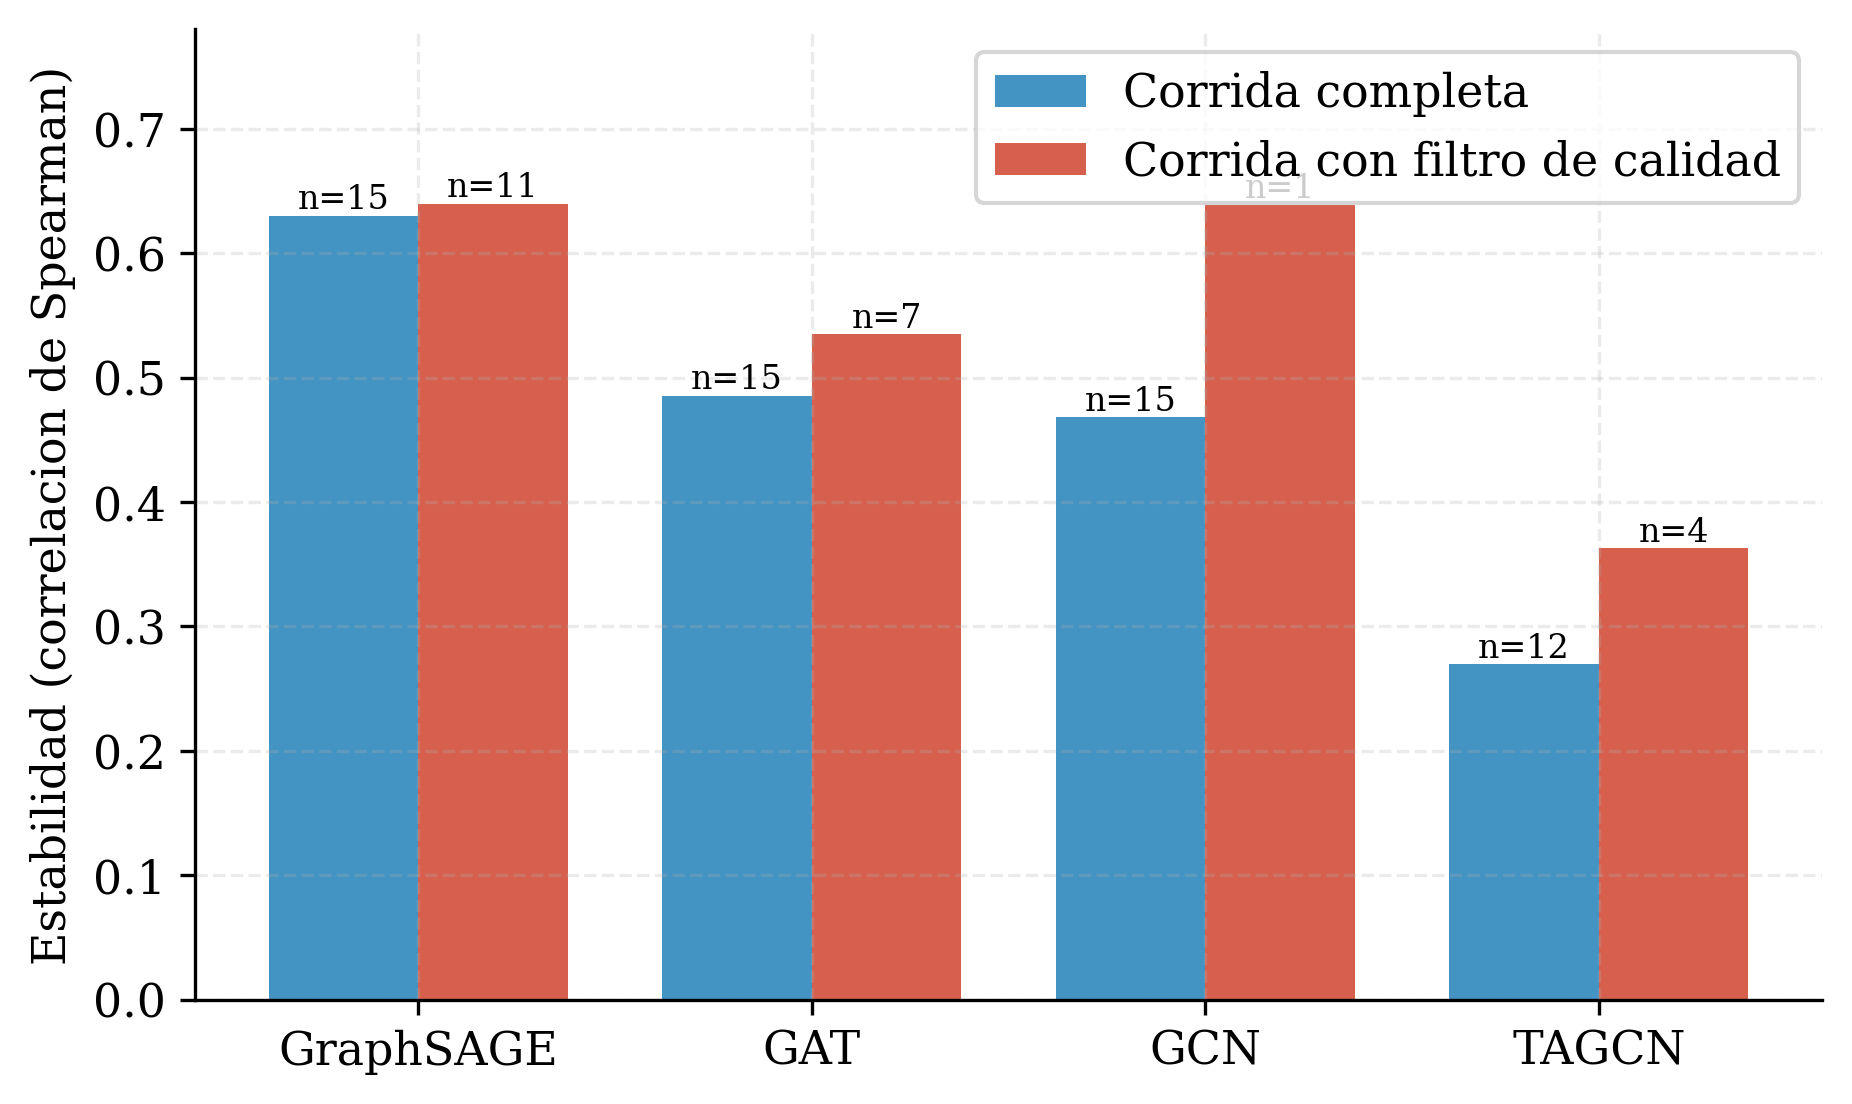
\includegraphics[width=\linewidth]{chapter_4/images_ch4/ranking_khop.png}
\end{column}
\end{columns}
\end{frame}

\begin{frame}{Robustez: qué sostiene esa partición}
\begin{columns}[T]
\begin{column}{0.54\textwidth}
\footnotesize
\begin{tabular}{lcc}
\toprule
\textbf{Contraste} & \textbf{Estadístico} & \textbf{$p$} \\
\midrule
Global (4 arquitecturas) & Kruskal-Wallis & $2{,}8\!\times\!10^{-5}$ \\
Grupo alto vs bajo & Mann-Whitney & $1{,}4\!\times\!10^{-6}$ \\
\midrule
Dentro del grupo alto & Kruskal-Wallis & $0{,}19$ \\
Dentro del grupo bajo & Kruskal-Wallis & $0{,}08$ \\
\bottomrule
\end{tabular}
\vspace{7pt}
\begin{itemize}\footnotesize
  \item Tamaño de efecto $\varepsilon^2 = 0{,}125$.
  \item IC95\,\% bootstrap: se solapan \textbf{dentro} de cada grupo, apenas se tocan \textbf{entre} grupos.
  \item La separación entre grupos sobrevive la corrección de \textbf{Holm} por comparaciones múltiples.
\end{itemize}
\end{column}
\begin{column}{0.44\textwidth}
\begin{block}{Reproducibilidad, en sentido preciso}
\footnotesize
Reentrenamos la matriz completa desde cero. Los \textbf{pesos no} se reproducen bit a bit (los \textit{scatter} en GPU acumulan con sumas atómicas).\\[4pt]
Las \textbf{conclusiones sí}: 25/60 sobre el filtro de calidad frente a 23/60, y la \textbf{misma partición}.
\end{block}
\vspace{2pt}
{\footnotesize\color{muted} Distinguir ambas cosas es, en sí mismo, una contribución metodológica.}
\end{column}
\end{columns}
\end{frame}

\begin{frame}{Resultado 1b: concordancia entre regímenes}
\begin{columns}[T]
\begin{column}{0.5\textwidth}
\begin{itemize}\small
  \item La ``inversión por densidad'' era un \textbf{artefacto} de la métrica.
  \item Corregida, Elliptic (disperso) \textbf{concuerda} con el sintético (denso).
  \item Y la coincidencia no es solo de orden: el eje sintético separa \textbf{los mismos dos grupos}, medido sobre datos y \textit{pipeline} independientes.
\end{itemize}
\vspace{4pt}
\begin{center}
\small Correlación de rangos entre regímenes\\[3pt]
{\color{coral}\Large\textbf{$-0{,}20$}} \; $\rightarrow$ \; {\color{amber}\Large\textbf{$+0{,}80$}}\\[2pt]
{\footnotesize métrica con bug \; $\rightarrow$ \; métrica corregida}\\[5pt]
{\footnotesize\color{muted} Sintético: GCN 0,97 y GAT 0,96 \; frente a \; GraphSAGE 0,89 y TAGCN 0,89}
\end{center}
\end{column}
\begin{column}{0.5\textwidth}
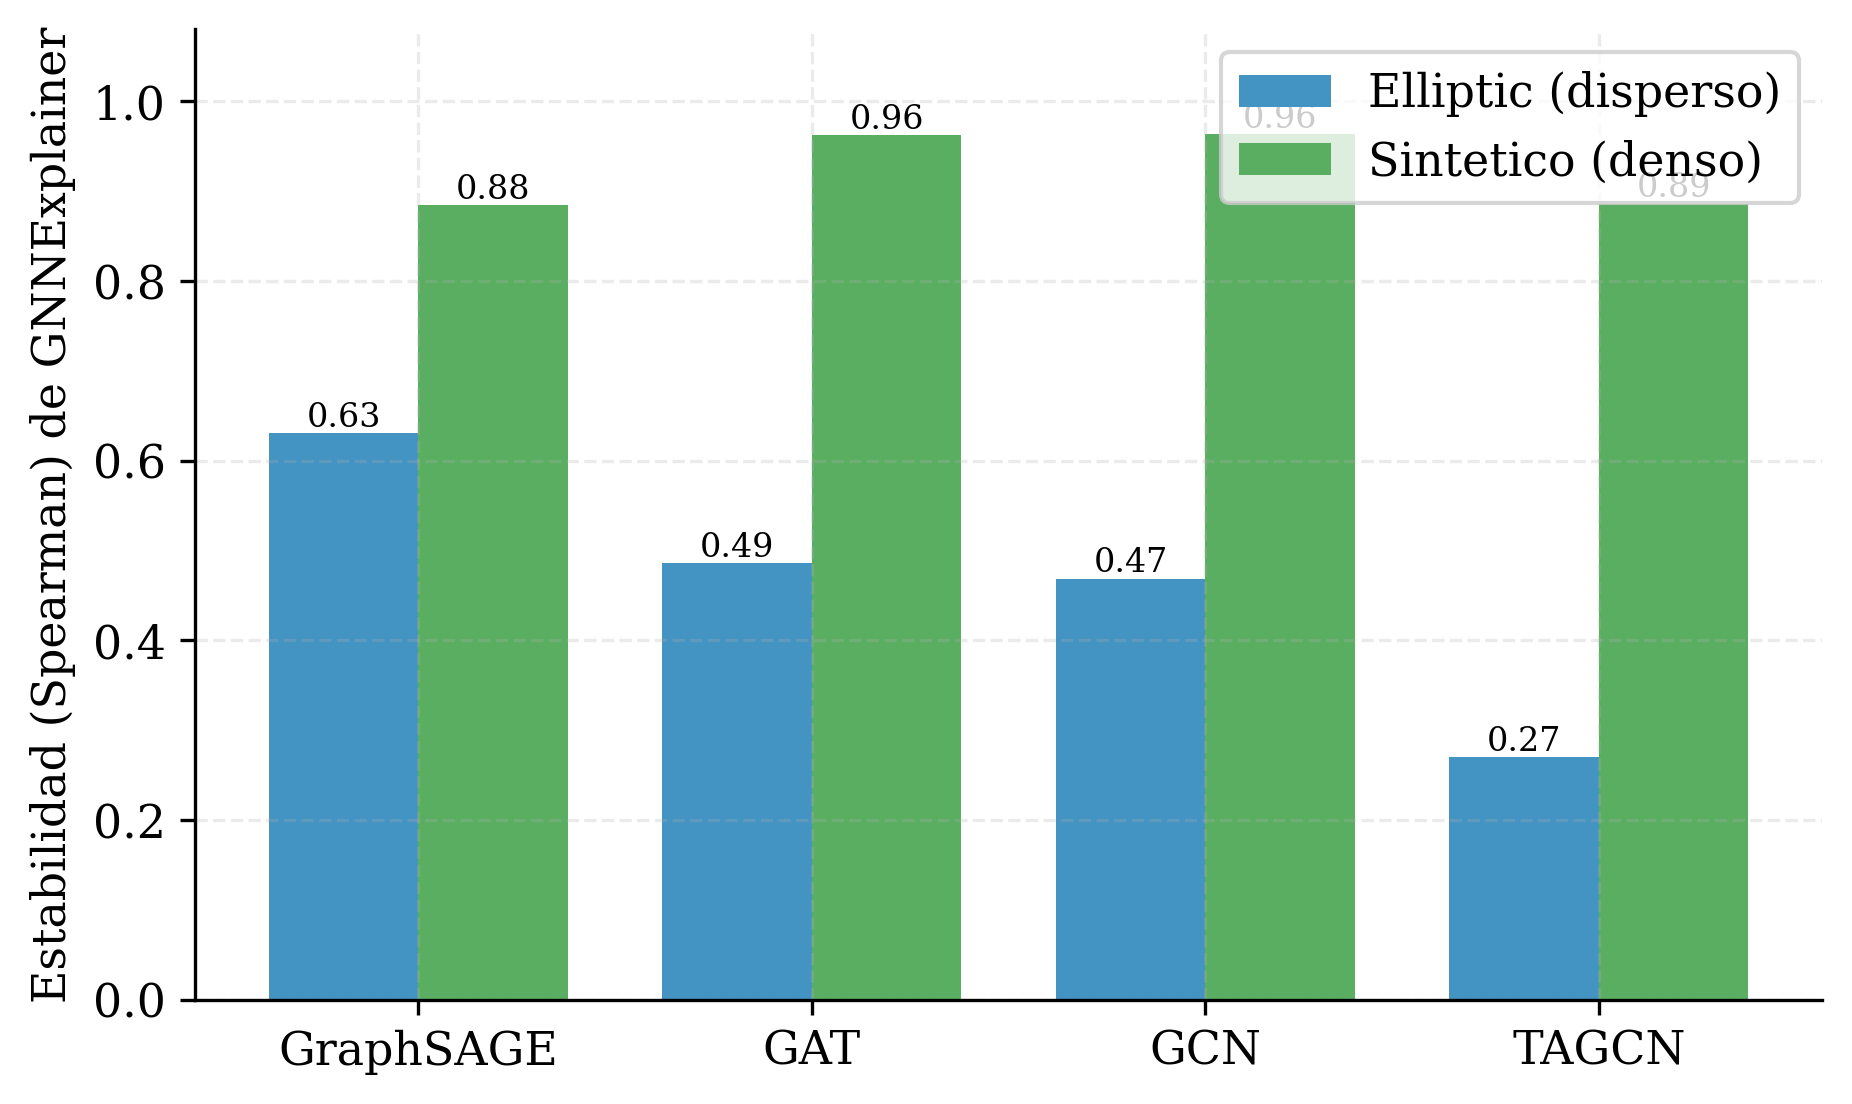
\includegraphics[width=\linewidth]{chapter_5/images_ch5/contraste_regimen.png}
\end{column}
\end{columns}
\end{frame}

\begin{frame}{Resultado 2: disociación plausibilidad / fidelidad}
\begin{columns}[T]
\begin{column}{0.52\textwidth}
\begin{itemize}\small
  \item \textbf{\color{teal}PGExplainer} recupera mejor el patrón: plausibilidad de aristas 0,80 vs 0,50, con 0,40 de azar (Wilcoxon $p\approx 2{,}6\times10^{-35}$)\dots
  \item \dots pero \textbf{\color{coral}colapsa en fidelidad}: 0,11 vs 0,56 de GNNExplainer.
  \item \textit{El explicador más ``plausible'' no es el más fiel.}
\end{itemize}
\end{column}
\begin{column}{0.48\textwidth}
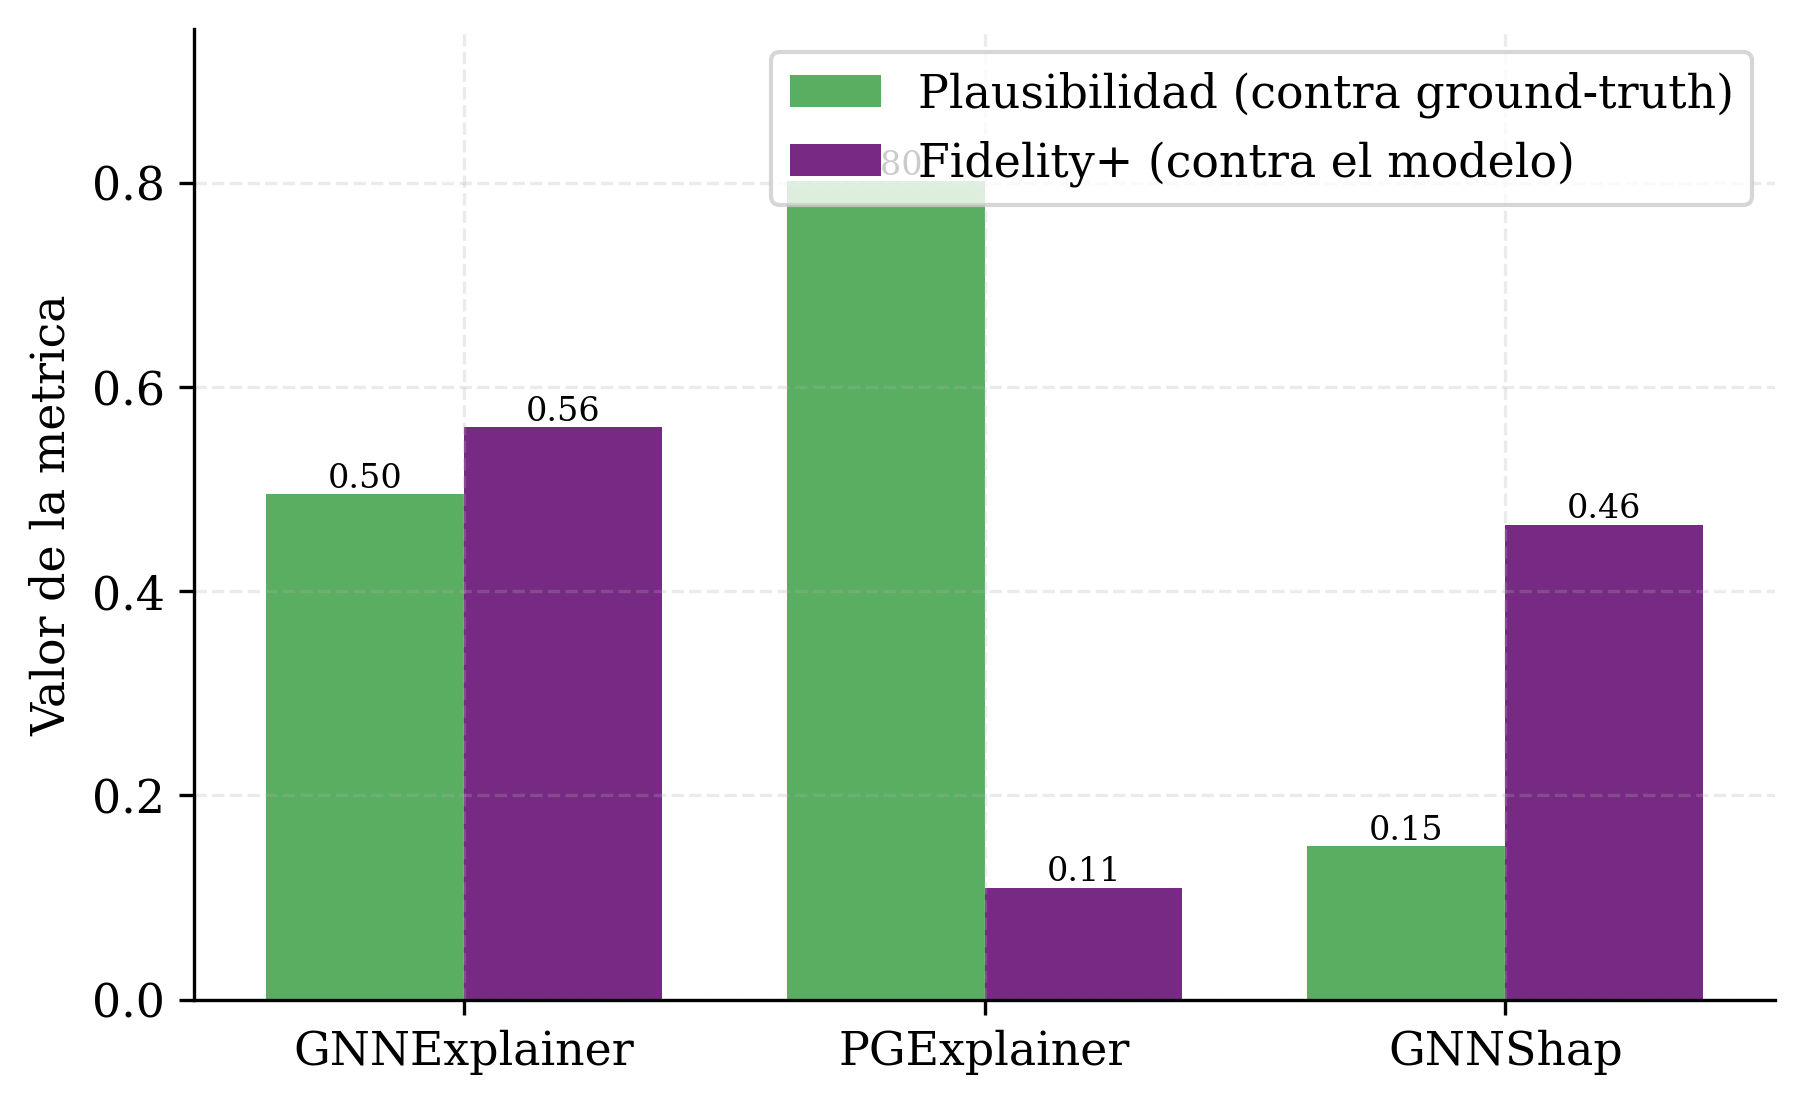
\includegraphics[width=\linewidth]{chapter_5/images_ch5/disociacion.png}
\end{column}
\end{columns}
\end{frame}

\begin{frame}{Resultado 3: el puente que no existe}
\begin{columns}[T]
\begin{column}{0.52\textwidth}
\begin{itemize}\small
  \item Nuestra hipótesis central: una explicación más estable señalaría mejor el patrón real.
  \item El dato dice que \textbf{no}. Correlación estabilidad--plausibilidad $r=-0{,}01$, con IC 95\,\% de $-0{,}038$ a $+0{,}011$.
  \item El intervalo \textbf{incluye el cero}: no hay relación, ni positiva ni negativa.
\end{itemize}
\vspace{4pt}
\small\textit{Es un no-resultado, y lo reportamos precisamente porque contradice lo que esperábamos.}
\end{column}
\begin{column}{0.48\textwidth}
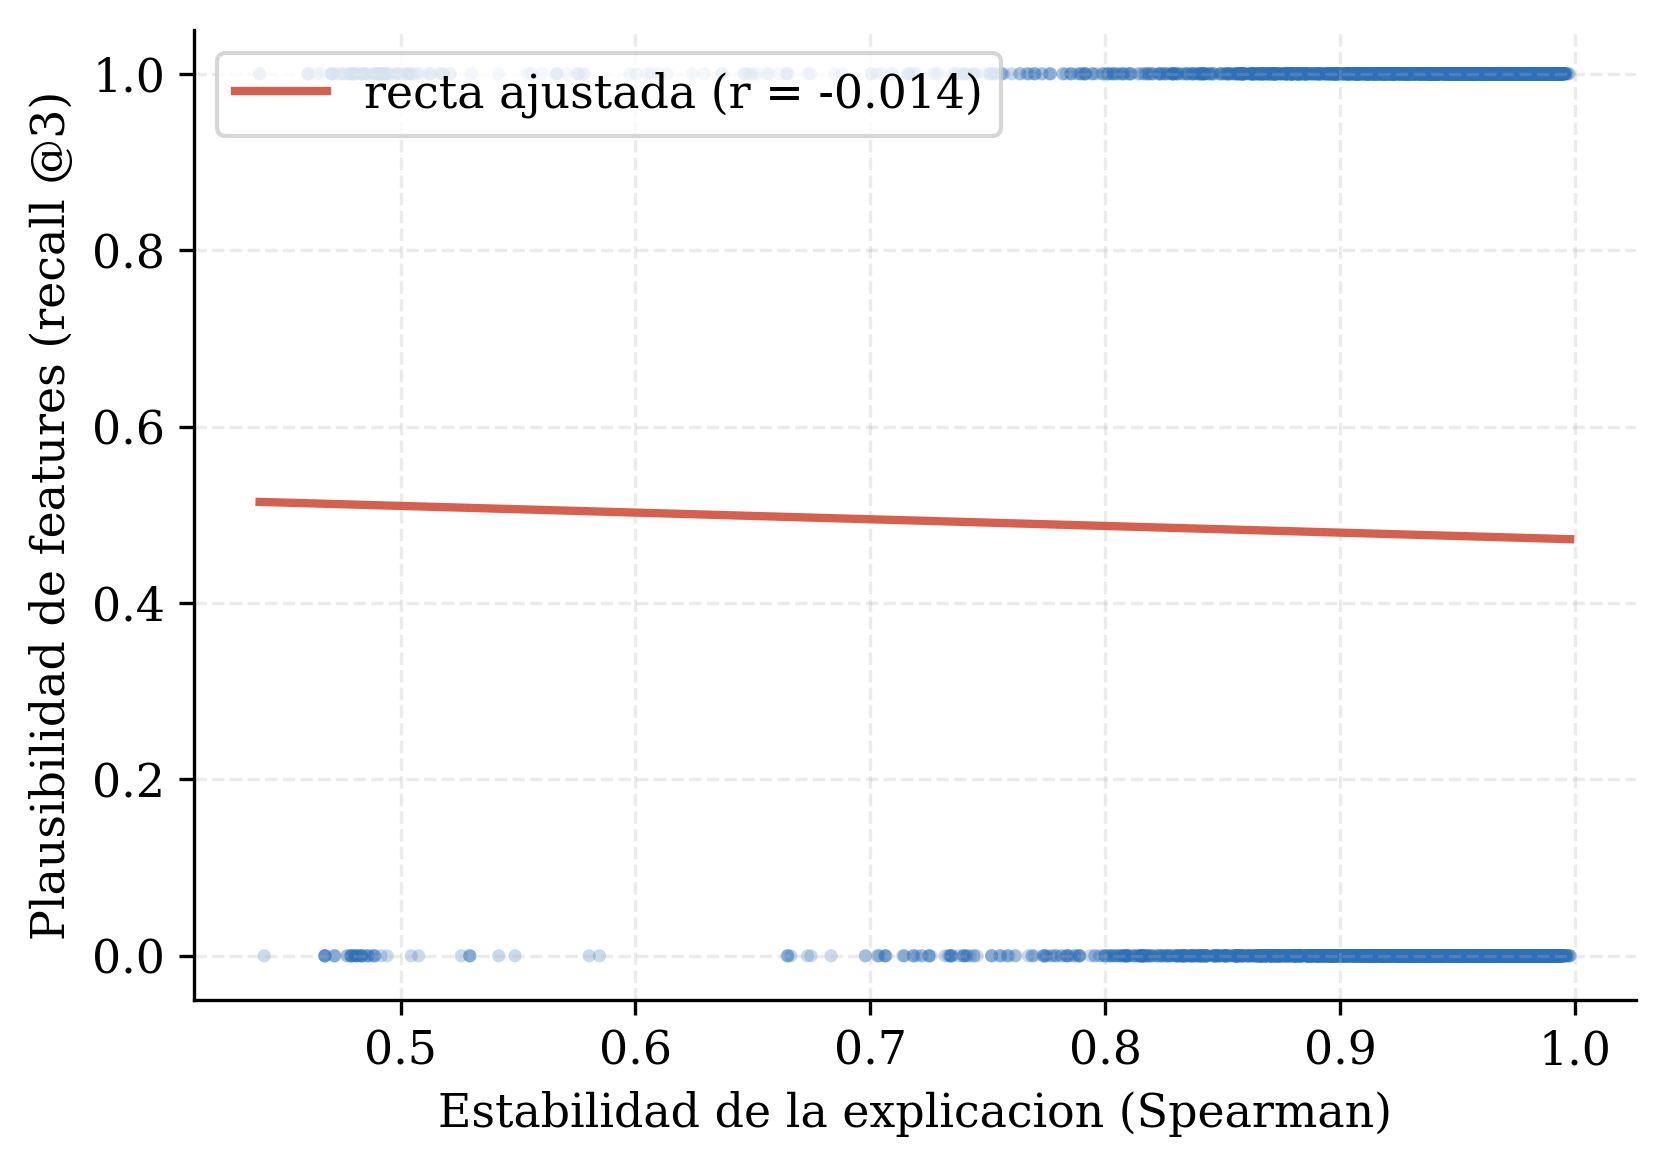
\includegraphics[width=\linewidth]{chapter_5/images_ch5/puente_nulo.png}
\end{column}
\end{columns}
\end{frame}

\begin{frame}{Resultado 4: el desbalance no gobierna la estabilidad}
\begin{columns}[T]
\begin{column}{0.5\textwidth}
\begin{itemize}\small
  \item Esperábamos degradación al agravarse el desbalance. El perfil es \textbf{plano}.
  \item Entre escenarios la estabilidad media apenas se mueve, de $0{,}709$ en el nativo a $0{,}741$ en 1:100: una amplitud total de \textbf{tres centésimas}.
  \item Sin punto de quiebre, sin pico en 1:50, sin paradoja del escenario nativo.
  \item El \textbf{balanceo} tampoco pesa: $\eta^2 < 0{,}02$ en las tres dimensiones.
\end{itemize}
\vspace{6pt}
\begin{block}{}
\footnotesize Implicación práctica: el balanceo puede elegirse por \textbf{rendimiento}, sin temer que degrade la interpretabilidad.
\end{block}
\end{column}
\begin{column}{0.5\textwidth}
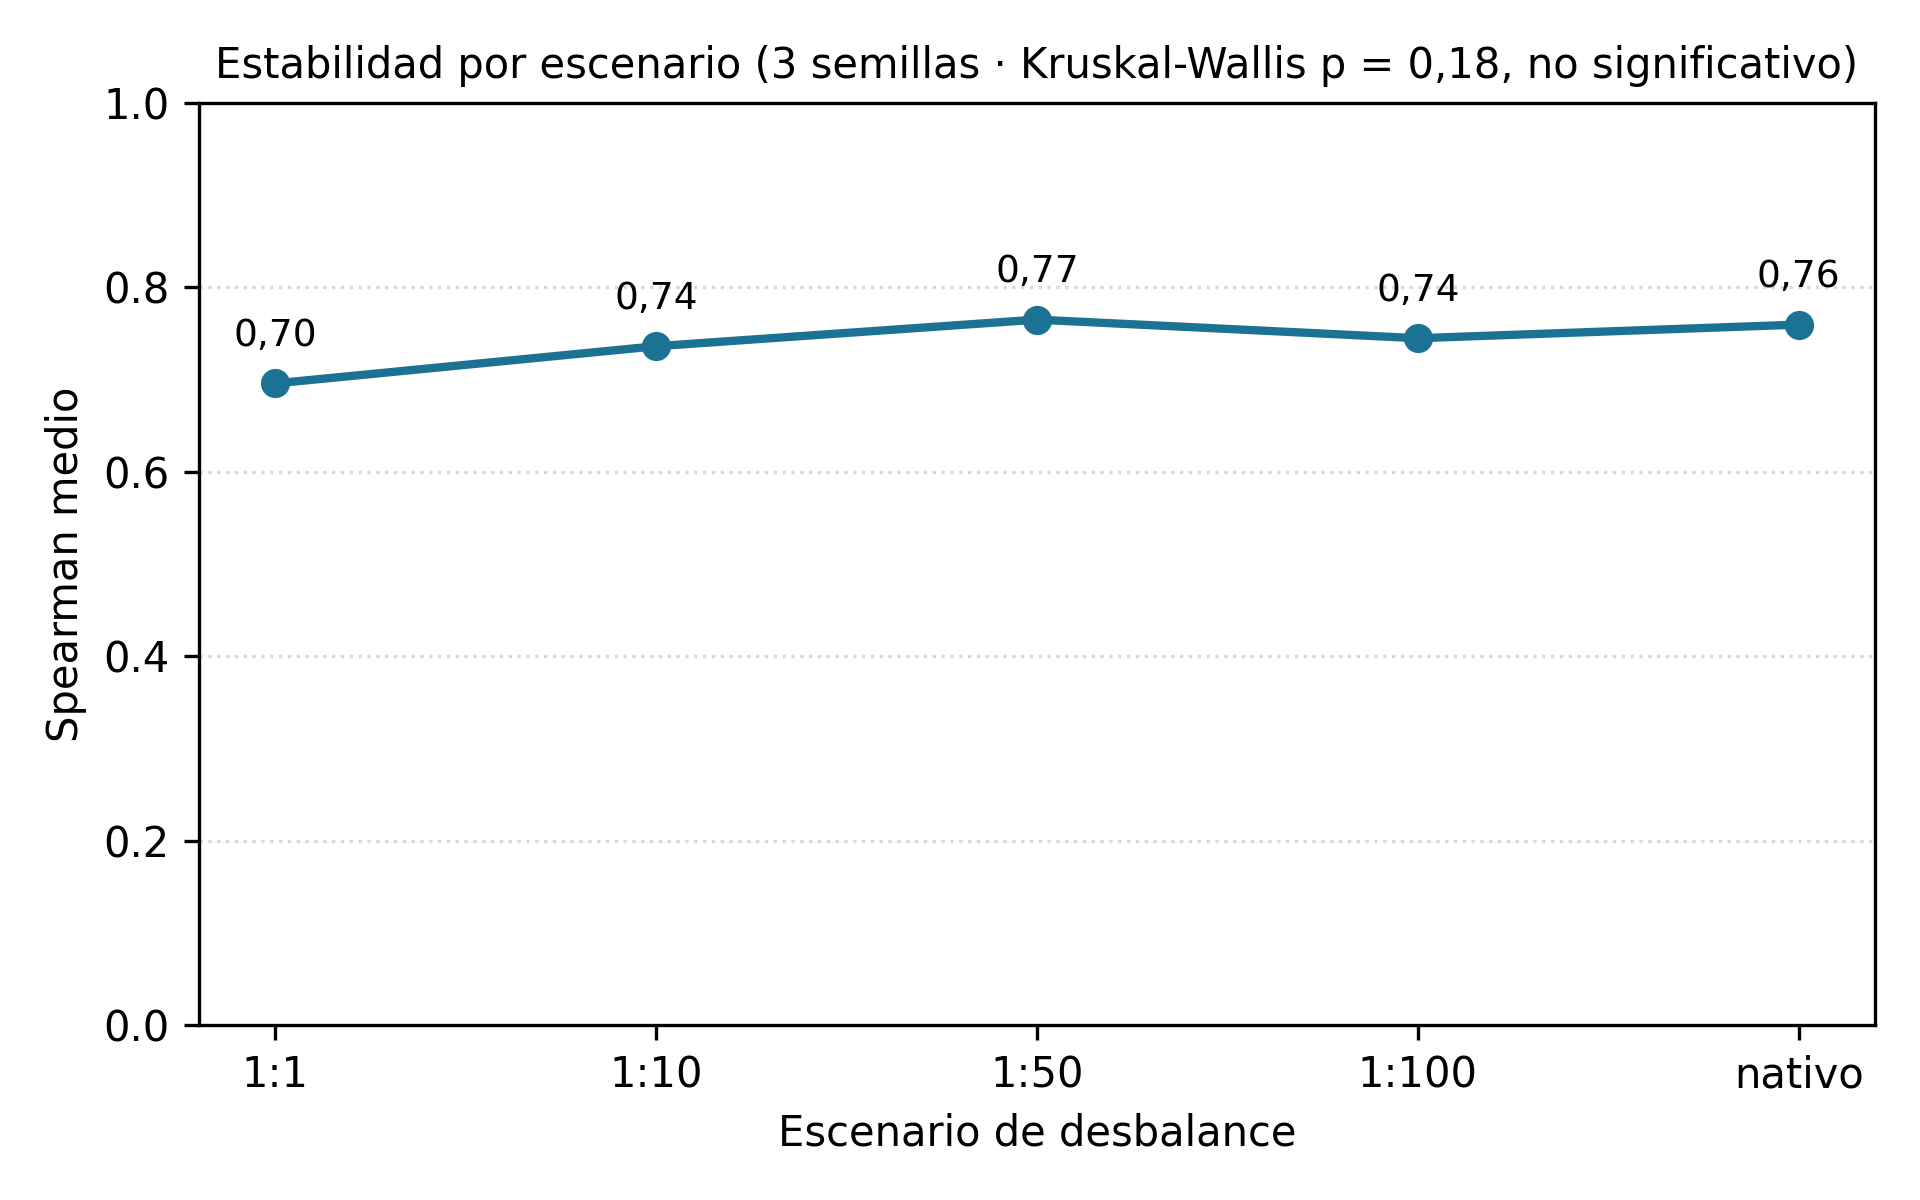
\includegraphics[width=\linewidth]{chapter_4/images_ch4/estabilidad_escenario.png}
\end{column}
\end{columns}
\end{frame}

\begin{frame}{Rendimiento y colapso validación $\rightarrow$ test}
\begin{columns}[T]
\begin{column}{0.33\textwidth}
\begin{block}{PR-AUC}\centering 0,367 \\ {\footnotesize\color{muted}validación}\\ $\rightarrow$ test \textbf{\color{coral}0,017}\end{block}
\end{column}
\begin{column}{0.33\textwidth}
\begin{block}{ROC-AUC}\centering 0,884 \\ {\footnotesize\color{muted}validación}\\ $\rightarrow$ test \textbf{\color{coral}0,653}\end{block}
\end{column}
\begin{column}{0.33\textwidth}
\begin{block}{Precision@50}\centering 0,657 \\ {\footnotesize\color{muted}validación}\\ $\rightarrow$ test \textbf{\color{coral}0,020}\end{block}
\end{column}
\end{columns}
\vspace{8pt}
\begin{center}\small
El \textbf{ROC-AUC es engañoso} bajo desbalance $\Rightarrow$ PR-AUC y precision@k como primarias.\\
La estabilidad se estudia sobre verdaderos positivos de \textbf{validación} (encuadre declarado).
\end{center}
\end{frame}

\begin{frame}{Rigor métrico: por qué PR-AUC y no ROC-AUC}
\begin{center}
\small
\renewcommand{\arraystretch}{1.35}
\begin{tabular}{lcc}
\toprule
\textbf{Métrica de ordenamiento} & \textbf{Validación} & \textbf{Test} \\
\midrule
ROC-AUC & 0,884 & 0,653 \\
\textbf{PR-AUC} & \textbf{0,367} & \textbf{0,017} \\
Precisión en los primeros 50 & 0,657 & 0,020 \\
Precisión en los primeros 100 & 0,640 & 0,022 \\
\bottomrule
\end{tabular}
\\[9pt]
\footnotesize
El ROC-AUC de 0,884 sugeriría un clasificador casi excelente. El PR-AUC de 0,367 sobre los mismos\\
modelos revela la dificultad real: bajo desbalance extremo, el eje de falsos positivos queda\\
dominado por la clase mayoritaria y permanece bajo aunque el modelo no distinga la clase rara.
\end{center}
\end{frame}

\begin{frame}{Las tres hipótesis, y qué pasó con cada una}
\begin{center}
\small
\renewcommand{\arraystretch}{1.7}
\begin{tabular}{p{0.44\textwidth}p{0.17\textwidth}p{0.30\textwidth}}
\toprule
\textbf{Lo que predijimos} & \textbf{Veredicto} & \textbf{La evidencia} \\
\midrule
\textbf{H1.} La estabilidad se degradaría al agravarse el desbalance. & \textcolor{coral}{\textbf{Refutada}} & Perfil plano: amplitud total de 0,03 entre escenarios (mín. 0,709 nativo, máx. 0,741 en 1:100). \\
\textbf{H2.} TAGCN sería la más estable, por su alcance multi-hop. & \textcolor{coral}{\textbf{Refutada}} & TAGCN queda en el grupo bajo en las 3 semillas. \\
\textbf{H3.} Un explicador más estable señalaría mejor el patrón. & \textcolor{coral}{\textbf{Refutada}} & Puente nulo: $r=-0{,}01$, IC incluye el cero. \\
\bottomrule
\end{tabular}
\\[10pt]
\footnotesize
Las tres se cayeron. \textbf{Ninguna se ocultó.}\\
Comprometerse con predicciones falsables antes de ver los datos es lo que permite que refutarlas sea un resultado, y no un fracaso.
\end{center}
\end{frame}

% ##################################################################### 5
\section{Conclusiones}

\begin{frame}{Los cuatro objetivos, respondidos}
\begin{center}
\footnotesize
\renewcommand{\arraystretch}{1.55}
\begin{tabular}{p{0.30\textwidth}p{0.62\textwidth}}
\toprule
\textbf{Objetivo} & \textbf{Respuesta} \\
\midrule
\textbf{O1.} Impacto del desbalance sobre la robustez explicativa & No es el factor dominante. El perfil es plano y el balanceo tiene efecto despreciable. La palanca real es el \textbf{explicador}. \\
\textbf{O2.} Resiliencia comparada de las 4 arquitecturas & No hay cuatro posiciones, hay \textbf{dos grupos}: alto (GAT, GCN) y bajo (GraphSAGE, TAGCN). La partición se replica en ambos regímenes de densidad. \\
\textbf{O3.} Impacto de las estrategias de balanceo & Despreciable sobre las tres dimensiones ($\eta^2 < 0{,}02$). Puede elegirse por rendimiento. \\
\textbf{O4.} Matriz de recomendación técnica & No existe una tríada óptima única. La recomendación es \textbf{condicional al propósito} de la auditoría. \\
\bottomrule
\end{tabular}
\end{center}
\end{frame}

\begin{frame}{Matriz de recomendación}
\begin{center}
\renewcommand{\arraystretch}{1.5}
\begin{tabular}{ll}
\toprule
\textbf{Objetivo operativo} & \textbf{Configuración} \\
\midrule
Auditabilidad / estabilidad & \textcolor{teal}{\textbf{grupo alto: GAT o GCN}} \\
Recuperar el patrón (plausibilidad) & \textcolor{seafoam}{\textbf{PGExplainer}} \\
Fidelidad al modelo & \textcolor{amber}{\textbf{GNNExplainer}} \\
Estabilidad interna del método & \textcolor{coral}{\textbf{GNNShap}} \\
\bottomrule
\end{tabular}
\\[8pt]
{\footnotesize\color{muted} La recomendación de arquitectura es \textbf{de grupo}, no de una arquitectura concreta:\\dentro del grupo alto la evidencia no distingue, así que la elección puede atender a coste o disponibilidad.}
\end{center}
\end{frame}

\begin{frame}{Contribuciones y limitaciones}
\begin{columns}[T]
\begin{column}{0.5\textwidth}
\begin{block}{Contribuciones}
\begin{itemize}\small
  \item Tres dimensiones independientes.
  \item Corrección de dos artefactos + dos \textit{bugs} de PGExplainer.
  \item Generador sintético con \textit{ground-truth} por arista.
  \item Reproducibilidad de \textbf{pesos} frente a la de \textbf{conclusiones}.
  \item Matriz de recomendación por objetivo.
\end{itemize}
\end{block}
\end{column}
\begin{column}{0.5\textwidth}
\begin{alertblock}{Limitaciones (declaradas)}
\begin{itemize}\small
  \item La inferencia fuerte proviene del eje sintético.
  \item El clasificador colapsa en test (\textit{shift} temporal).
  \item Un solo \textit{dataset} real, anonimizado.
  \item Con 3 semillas se sostiene el \textbf{grupo}, no el orden fino dentro de él.
\end{itemize}
\end{alertblock}
\end{column}
\end{columns}
\end{frame}

% ---- cierre ----
{\setbeamercolor{background canvas}{bg=navy}
\begin{frame}[plain,noframenumbering]
\vspace{0.3cm}\par
\hspace*{0.4cm}{\color{amber}\rule{1cm}{2.5pt}}\par\vspace{8pt}
\hspace*{0.4cm}{\color{white}\Large\bfseries Conclusiones}\par\vspace{10pt}
\hspace*{0.4cm}\begin{minipage}{0.9\textwidth}
{\color{white}\small
\begin{itemize}
  \item Estabilidad $\neq$ plausibilidad $\neq$ fidelidad: el mejor explicador depende del objetivo.
  \item Con la medición corregida, datos reales y sintéticos cuentan una historia coherente (GAT/GCN estables).
  \item La estabilidad de una explicación depende del protocolo de evaluación, no solo del método.
\end{itemize}}
\vspace{4pt}\par
{\color{white!85}\small \textbf{Trabajo futuro:} Elliptic2, AMLSim, GNNs temporales, GraphSMOTE.}
\end{minipage}\par\vspace{16pt}
\begin{center}
{\color{white}\Large\bfseries Gracias \textperiodcentered\ Preguntas}\par\vspace{3pt}
{\color{white!80}\small Alejandro Gómez Huertas \textperiodcentered\ Juan Diego Garzón Ovalle}
\end{center}
\end{frame}}

% ##################################################################### RESPALDO
\appendix
\section{Respaldo (solo si se pregunta)}

\begin{frame}{Respaldo \textperiodcentered\ estabilidad por semilla de modelo}
\begin{center}
\small
\renewcommand{\arraystretch}{1.3}
\begin{tabular}{lccccc}
\toprule
\textbf{Arquitectura} & \textbf{s42} & \textbf{s43} & \textbf{s44} & \textbf{Media} & \textbf{IC95\,\%} \\
\midrule
GAT       & 0,766 & 0,789 & 0,790 & \textbf{0,782} & [0,758; 0,805] \\
GCN       & 0,783 & 0,733 & 0,757 & \textbf{0,758} & [0,724; 0,787] \\
GraphSAGE & 0,756 & 0,713 & 0,738 & 0,735 & [0,710; 0,756] \\
TAGCN     & 0,586 & 0,693 & 0,736 & 0,672 & [0,632; 0,717] \\
\bottomrule
\end{tabular}
\\[9pt]
\footnotesize
\textbf{GAT y GCN se permutan} entre semillas: por eso no nombramos un ganador único.\\
\textbf{TAGCN} tiene la mayor dispersión (dt $0{,}077$, el triple que las demás): su lugar en el grupo bajo es firme, su valor central admite margen.
\end{center}
\end{frame}

\begin{frame}{Respaldo \textperiodcentered\ detalle estadístico de la partición}
\begin{center}
\footnotesize
\renewcommand{\arraystretch}{1.25}
\begin{tabular}{lcc}
\toprule
\textbf{Wilcoxon pareado} & \textbf{Elliptic} & \textbf{Sintético} \\
\midrule
GAT vs GCN \hfill \textit{(dentro del grupo alto)} & 0,165 & 0,0013 \\
GraphSAGE vs TAGCN \hfill \textit{(dentro del grupo bajo)} & 0,096 & 0,519 \\
\midrule
GAT vs GraphSAGE & 0,0033 & $<10^{-4}$ \\
GAT vs TAGCN & $<10^{-4}$ & $<10^{-4}$ \\
GCN vs GraphSAGE & 0,047 & $<10^{-4}$ \\
GCN vs TAGCN & 0,0067 & $<10^{-4}$ \\
\bottomrule
\end{tabular}
\\[8pt]
\footnotesize
La única diferencia intragrupo significativa es GCN sobre GAT en el eje sintético,\\
por un margen de \textbf{0,006} sin relevancia práctica, detectable solo por el mayor $n$ de ese eje.
\end{center}
\end{frame}

\begin{frame}{Respaldo \textperiodcentered\ ¿por qué GNNExplainer para el ranking?}
\begin{center}
\small
\renewcommand{\arraystretch}{1.3}
\begin{tabular}{lcccc}
\toprule
\textbf{Explicador (Elliptic)} & \textbf{GAT} & \textbf{GCN} & \textbf{GraphSAGE} & \textbf{TAGCN} \\
\midrule
\textbf{\color{teal}GNNExplainer} & 0,78 & 0,78 & 0,74 & 0,58 \\
PGExplainer & 0,00 & 0,00 & 0,00 & 0,00 \\
GNNShap & 0,96 & 0,98 & 0,94 & 0,97 \\
\bottomrule
\end{tabular}
\\[10pt]
\footnotesize
GNNExplainer es el \textbf{único que discrimina} arquitecturas en Elliptic. PGExplainer \textbf{degenera} (Spearman nulo en las cuatro) y GNNShap se \textbf{satura} en torno a $0{,}95$, indistinguible entre arquitecturas, igual que el índice de Jaccard.\\[4pt]
\textbf{\color{teal}La elección de GNNExplainer no es arbitraria:} es el único explicador con señal de estabilidad medible en este eje, y además el común a los dos ejes.
\end{center}
\end{frame}

\end{document}
